% This text is proprietary.
% It's a part of presentation made by myself.
% It may not used commercial.
% The noncommercial use such as private and study is free
% Dec 2007
% Author: Sascha Frank 
% University Freiburg 
% www.informatik.uni-freiburg.de/~frank/
%
% 
\documentclass{beamer}
\usepackage[utf8]{inputenc}
\usepackage[english]{babel}
\usepackage{amsmath}
\usepackage{amsfonts}
\usepackage{amssymb}
\usepackage{graphicx}
\usepackage{empheq}
\usepackage{biblatex}
\usepackage{mathrsfs}
 
%\usepackage{calligra}
%\usepackage{calrsfs}
\addbibresource{library.bib}
\usepackage[listings,theorems]{tcolorbox}

\setbeamertemplate{navigation symbols}{}

\setbeamercolor{frametitle}{fg=black,bg=white}
\setbeamercolor{title}{fg=black,bg=white!85!blue}
%\usetheme{Boadilla}
\usetheme{Szeged}


\makeatletter
    \newenvironment{withoutheadline}{
        \setbeamertemplate{headline}[default]
        \def\beamer@entrycode{\vspace*{-\headheight}}
    }{}
\makeatother

\beamersetuncovermixins{\opaqueness<1>{25}}{\opaqueness<2->{15}}
\begin{document}

%==============================================================
\author[]{H. Aghakhani, A. K. Patra and E. Spiller}
\title{Construction of Gaussian
Surrogate Process Using Numerical
and Modeling Error Uncertainty}
\institute{SIAM CSE 2015}

\frame{\titlepage} 
\frame{\frametitle{Table of contents}\tableofcontents} 

%=============================================================
\section{Adjoint Definition and Derivation} 
\begin{withoutheadline}
\begin{frame}\frametitle{Adjoint Definition} 
Let: 
\begin{itemize}
\item Let $U$ and $V$ be two vector spaces, and $L$ be a linear operator that maps any $u \in U$ into $v \in V$.
\item $<\cdot,\cdot>$ be a bilinear map that maps any two vectors like $u,v$ two a real number, $U \times V \rightarrow  \mathbb{R}$.
\end{itemize}
Then the adjoint operator, $L^*$, of $L$ is defined:\\
$<Lu,v> = <u,L^*v>$.
\end{frame}
\end{withoutheadline}
%=============================================================
\begin{withoutheadline}
\begin{frame}\frametitle{Discrete Adjoint} 
Assume:
\begin{itemize}
\item $R(U,\alpha)$ as a system of governing equations,
\item $U$ is the solution vector, 
\item $\alpha$ is the vector of design parameters.
\end{itemize}
\vspace{.1in}
The object is to minimize \hspace{.05 in} J$(U,\alpha)$ \hspace{.1 in} subject to \hspace{.1 in} $R(U,\alpha)=0$

\end{frame}
\end{withoutheadline}
%=============================================================
\begin{withoutheadline}
\begin{frame}\frametitle{Discrete Adjoint Cont.} 

With writing the variation of the functional and governing equation w.r.t design parameters, we will have:
       
 \begin{displaymath}\pause 
 \frac{dJ}{d \alpha} = \frac{\partial J}{\partial U} \frac{d U}{d \alpha} + \frac{\partial J}{\partial \alpha} 
 \end{displaymath}
and:
  \begin{displaymath}\pause 
 \frac{\partial R}{\partial U} \frac{d U}{d \alpha} + \frac{\partial R}{\partial \alpha} = 0.
 \end{displaymath}
 \pause 
Now,if we replace $\frac{d U}{d \alpha}$ from the second equation into the first equation, we have:
\begin{displaymath}
 \frac{dJ}{d \alpha} = - \frac{\partial J}{\partial U} (\frac{\partial R}{\partial U})^{-1} \frac{\partial R}{\partial \alpha}  
+ \frac{\partial J}{\partial \alpha}
 \end{displaymath} 

\end{frame}
\end{withoutheadline}

%=============================================================
\begin{withoutheadline}
\begin{frame}[label=main]
\frametitle{Sensitivity Computation} 

Assume that n is the size of vector U, and m is the size of vector $\alpha$:
\pause
 \begin{displaymath}
dJ_{scalar}=\underbrace{- \left[\frac{\partial J}{\partial U}
 \right]_{1\times n} 
 \left[\frac{\partial R}{\partial U}^{-1} \right]_{n \times n} 
 \left[ \frac{\partial R}{\partial \alpha} \right]_{n \times m}  d \alpha_{m \times 1}}_\text{scalar}  + \underbrace{
 \left[\frac{\partial J}{\partial \alpha} \right] _{1\times m} d\alpha_{m\times 1}}_\text{scalar}
\end{displaymath}
 \pause
Above sensitivity can be computed in two ways:

\begin{enumerate}
\item Forward mode: first computes $(\frac{\partial R}{\partial U})^{-1} \frac{\partial R}{\partial \alpha}$
\pause
\item Adjoint mode: first computes $\frac{\partial J}{\partial U} (\frac{\partial R}{\partial U})^{-1} \rightarrow (\frac{\partial R}{\partial U})^{T} v = \frac{\partial J}{\partial U} ^ T, \ \ v$ is adjoint solution 
\end{enumerate}
\hyperlink{supplemental}{\beamerbutton{Adjoint definition}}
\pause

\begin{tcolorbox}[colback=blue!5,colframe=blue!75!black,title=Advantage of Adjoint:]
  If the number of design parameters are more than the objective functionals, then the computational cost of the adjoint is much lower than the forward method. 
\end{tcolorbox}


\end{frame}
\end{withoutheadline}
%=============================================================
\begin{withoutheadline}
\begin{frame}\frametitle{Computing Adjoint} 
To solve adjoint equation we need Transpose of Jacobian Matrix:
%{\tcbhighmath[colback=blue!2!white,arc=0pt,outer arc=0pt,toprule=0pt]}
\begin{empheq}[box=\fbox]{align*}
\left(\frac{\partial R}{\partial U}\right)^{T} v = \frac{\partial J}{\partial U} ^ T
\end{empheq}

TITAN2D uses Godunov finite volume with Euler explicit time scheme, so the descritized form of equations are:

\begin{displaymath}
 U_i^{n+1} = U_i^n - 
 \frac{\bigtriangleup t}{\bigtriangleup x} 
 \{F_{i+\frac{1}{2}}^n - F_{i-\frac{1}{2}}^n \}
 - \frac{\bigtriangleup t}{\bigtriangleup y} 
 \{G_{i+\frac{1}{2}}^n - G_{i-\frac{1}{2}}^n \}
 \end{displaymath}

  \begin{displaymath}
     \left(\frac{\partial R}{\partial U}\right)^{T}_{m \times m} = K_{ij}
  \end{displaymath} 
where  m is the number of time steps, and each $K_{ij}$ is a 
\end{frame}
\end{withoutheadline}
%=============================================================
\begin{withoutheadline}
\begin{frame}\frametitle{Computing Adjoint Cont.} 

For Euler explicit:
      \begin{displaymath}
        K_{i,i} = I \hspace{.15 in} \text{and} \hspace{.15 in} K_{i,i+1}= (\frac{\partial R_p^{i+1}}{\partial U_q^i})^T,
    \end{displaymath} 
    \begin{itemize}
    \item p and q are degrees of freedom
    \item rest of  the components are zero
    \item depend on the stencil is used. K matrices are also block bounded
    \end{itemize}

\begin{displaymath}
   (\frac{\partial R}{\partial U})_{m \times m}^T =
   \begin{pmatrix}
  I & K_{1,2}        &         &               &          \\
    & I              & K_{2,3} & \text{\huge0} &          \\
    &                & \ddots  & \ddots        &          \\
    & \text{\huge0}  &         & I             & K_{m-1,m}\\
    &                &         &               & I
 \end{pmatrix}
  \end{displaymath}  
  
  
\end{frame}
\end{withoutheadline}
%=============================================================
\begin{withoutheadline}
\begin{frame}\frametitle{Computing Adjoint Cont.} 
\begin{tcolorbox}[colback=blue!5,colframe=blue!75!black,title= Important conclusion:]
To compute adjoint for an explicit system, there is no need to solve a system of equation, and adjoint solution can be found marching backward in time.
\end{tcolorbox}

  \begin{displaymath}
  \begin{aligned}
 v_1 + K_{1,2} v_2 &=\left(\frac{\partial J}{\partial U}\right)_1^T \\
 &\vdots\\
 v_{m-1} + K_{m-1,m} v_m &=\left(\frac{\partial J}{\partial U}\right)_{m-1}^T \\
v_m &=\left(\frac{\partial J}{\partial U}\right)_m^T
 \end{aligned}
\end{displaymath}

\end{frame}
\end{withoutheadline}
%=============================================================
\section{Error Estimation}
\begin{withoutheadline}
\begin{frame}\frametitle{Error Estimation} 
The goal is to minimize the numerical error due to mesh size on the objective functional $ J(Q) $, given the solution on the coarse mesh $ J(Q_H) $.\\
With Taylor expansion we can write
\footfullcite{Nemec2008}:
\begin{displaymath}
J(Q_h) \approx  J(Q^H_h) - \underbrace{(\psi^H_h)^T R(Q^H_h)}_\text{Adjoint correction term} - 
\underbrace{(\psi_h - \psi^H_h)^T R(Q^H_h)}_\text{Remaining term},
\end{displaymath}
where $ J(Q_h) $ is the functional value on a finer mesh, and all $\square^H_h$ is the projection of $\square$ from the coarse mesh to the fine mesh.
\end{frame}
\end{withoutheadline}
%=============================================================
\begin{withoutheadline}
\begin{frame}\frametitle{Error Estimation Cont.} 
So to compute the error $ \varepsilon = |J(Q) - J(Q_H)| $:
\begin{itemize}
\item we have to first find $\psi_h$.
\item since computing $\psi_h$ is not reasonable to just compute the error we approximate it with higher order construction.
\end{itemize}
Consequently:

\begin{displaymath}
J(Q_h) \approx  J(Q_L) - (\psi_L)^T R(Q_L) - (\psi_L - \psi_C)^T R(Q_L),
\end{displaymath}

where $\square_L$, $\square_C$ represent linear and constant reconstruction respectively.

\end{frame}
\end{withoutheadline}
%=============================================================
\section{Results}

\begin{withoutheadline}
\begin{frame}\frametitle{Case 1: Burger's Equation} 

\begin{displaymath}
\begin{aligned}
R(x,t)&=\frac{\partial u}{\partial t}+\frac{\alpha}{2}\frac{\partial u^2}{\partial x}=0, \hspace{.25in} x\in (-1,1), \ \ t \in (0,1) ,\\
u(x,0)&=\beta \ cos (\frac{\pi}{2}  x) ,\\
u(1,t)&=0,\\
J&=0.5\int_T \int_x u^2 \ dx \ dt,
\end{aligned}
\end{displaymath}
where $ \alpha $ and $ \beta $ are uncertain parameters, and are selected from $\mathscr{N}(1,0.1)$.

\end{frame}
\end{withoutheadline}
%=============================================================
\begin{withoutheadline}
\begin{frame}\frametitle{Case 1: Results} 
Results are for a Monte Carlo simulation with 10,000 samples:\\
\center{Functional of interest as a function of advection coefficient}
\begin{figure}
\center 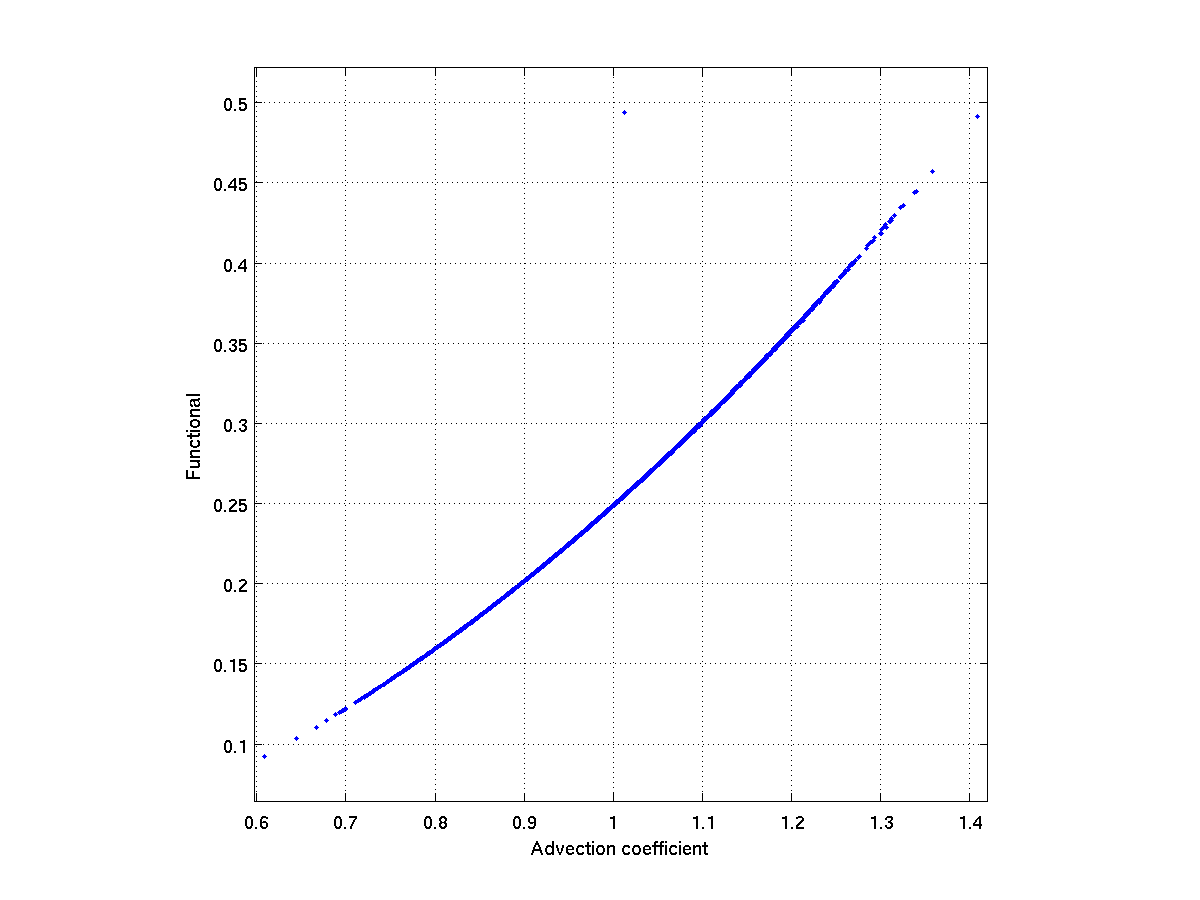
\includegraphics[width=.8\textwidth]{func_advec.png}
\end{figure}

\end{frame}
\end{withoutheadline}
%=============================================================
\begin{withoutheadline}
\begin{frame}\frametitle{Case 1: Results} 

\center{Functional of interest as a function of initial condition uncertain coefficient}
\begin{figure}
\center 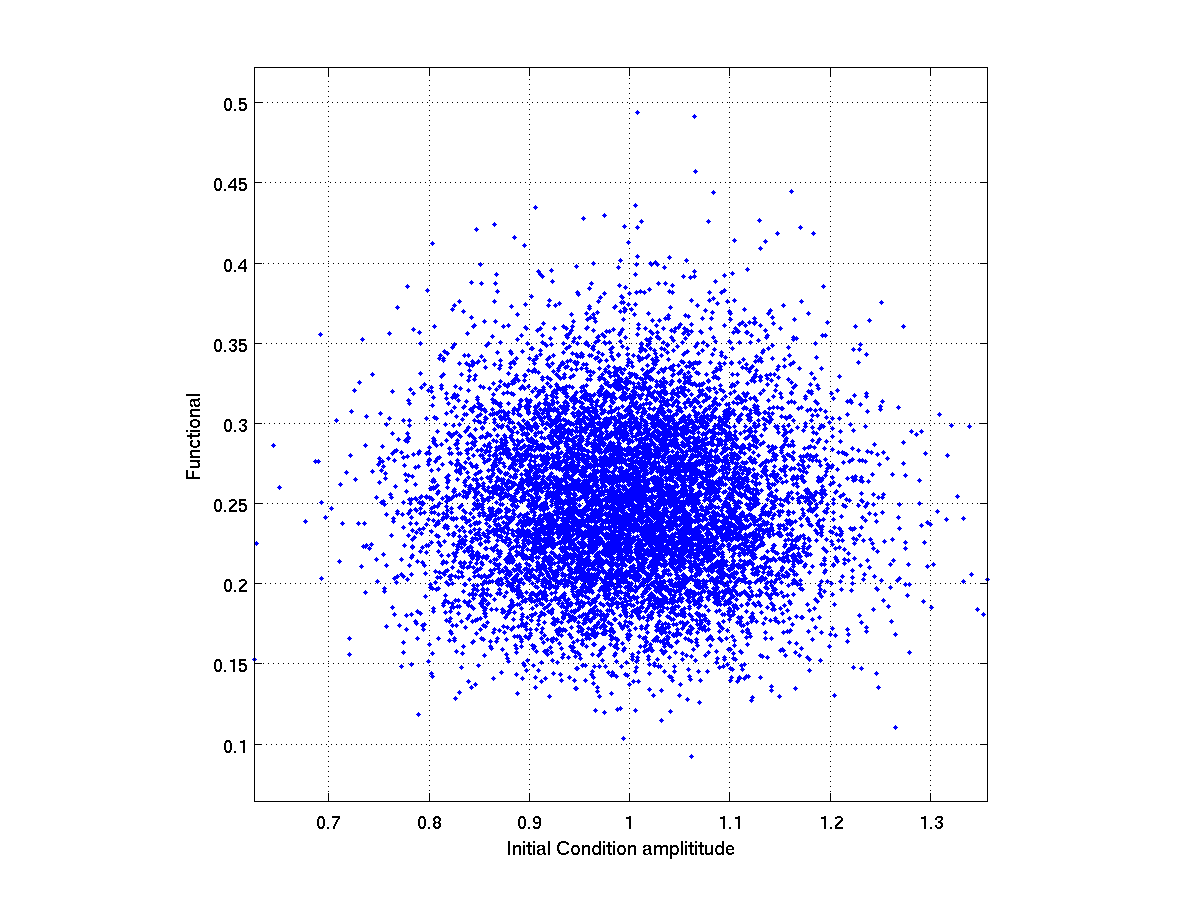
\includegraphics[width=.8\textwidth]{func_init.png}
\end{figure}
\end{frame}
\end{withoutheadline}
%=============================================================
\begin{withoutheadline}
\begin{frame}\frametitle{Case 1: Results} 

\center{Error at final stage as a function of advection coefficient}
\begin{figure}
\center 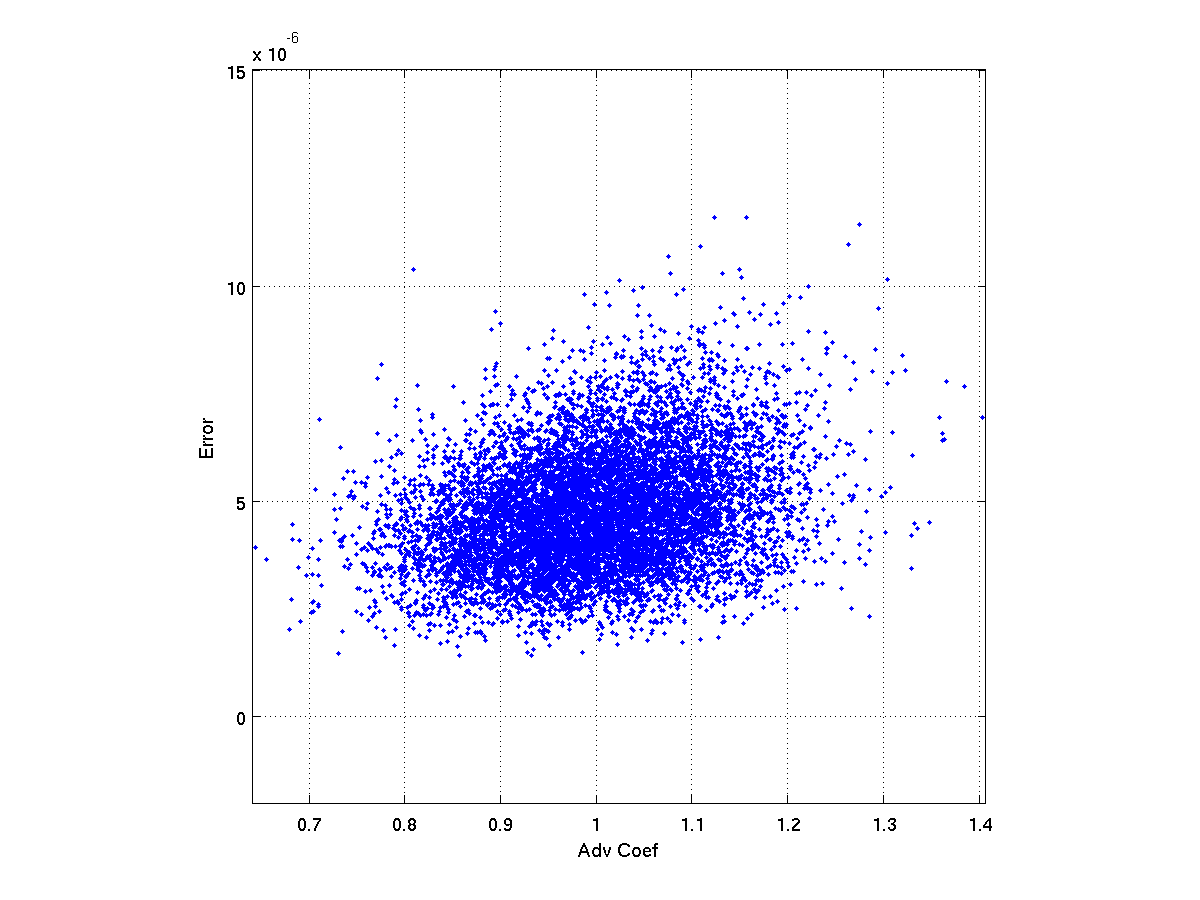
\includegraphics[width=.8\textwidth]{err_advec.png}
\end{figure}
\end{frame}
\end{withoutheadline}
%=============================================================
\begin{withoutheadline}
\begin{frame}\frametitle{Case 1: Results} 

\center{Error at final stage as a function of initial condition uncertain coefficient}
\begin{figure}
\center 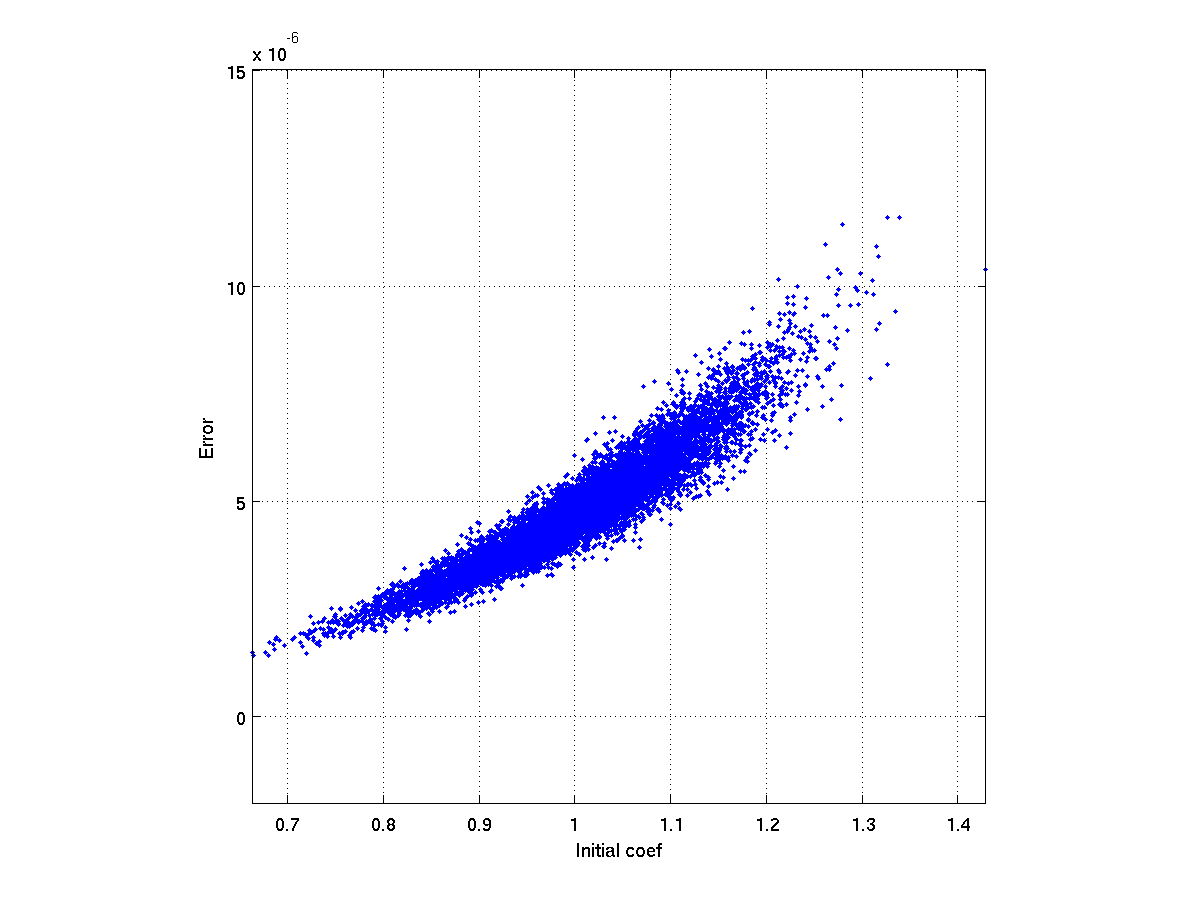
\includegraphics[width=.8\textwidth]{err_init.png}
\end{figure}

\end{frame}
\end{withoutheadline}
%=============================================================
\begin{withoutheadline}
\begin{frame}\frametitle{Case 1: Results} 


\center{Emulator result}
\begin{figure}
\center 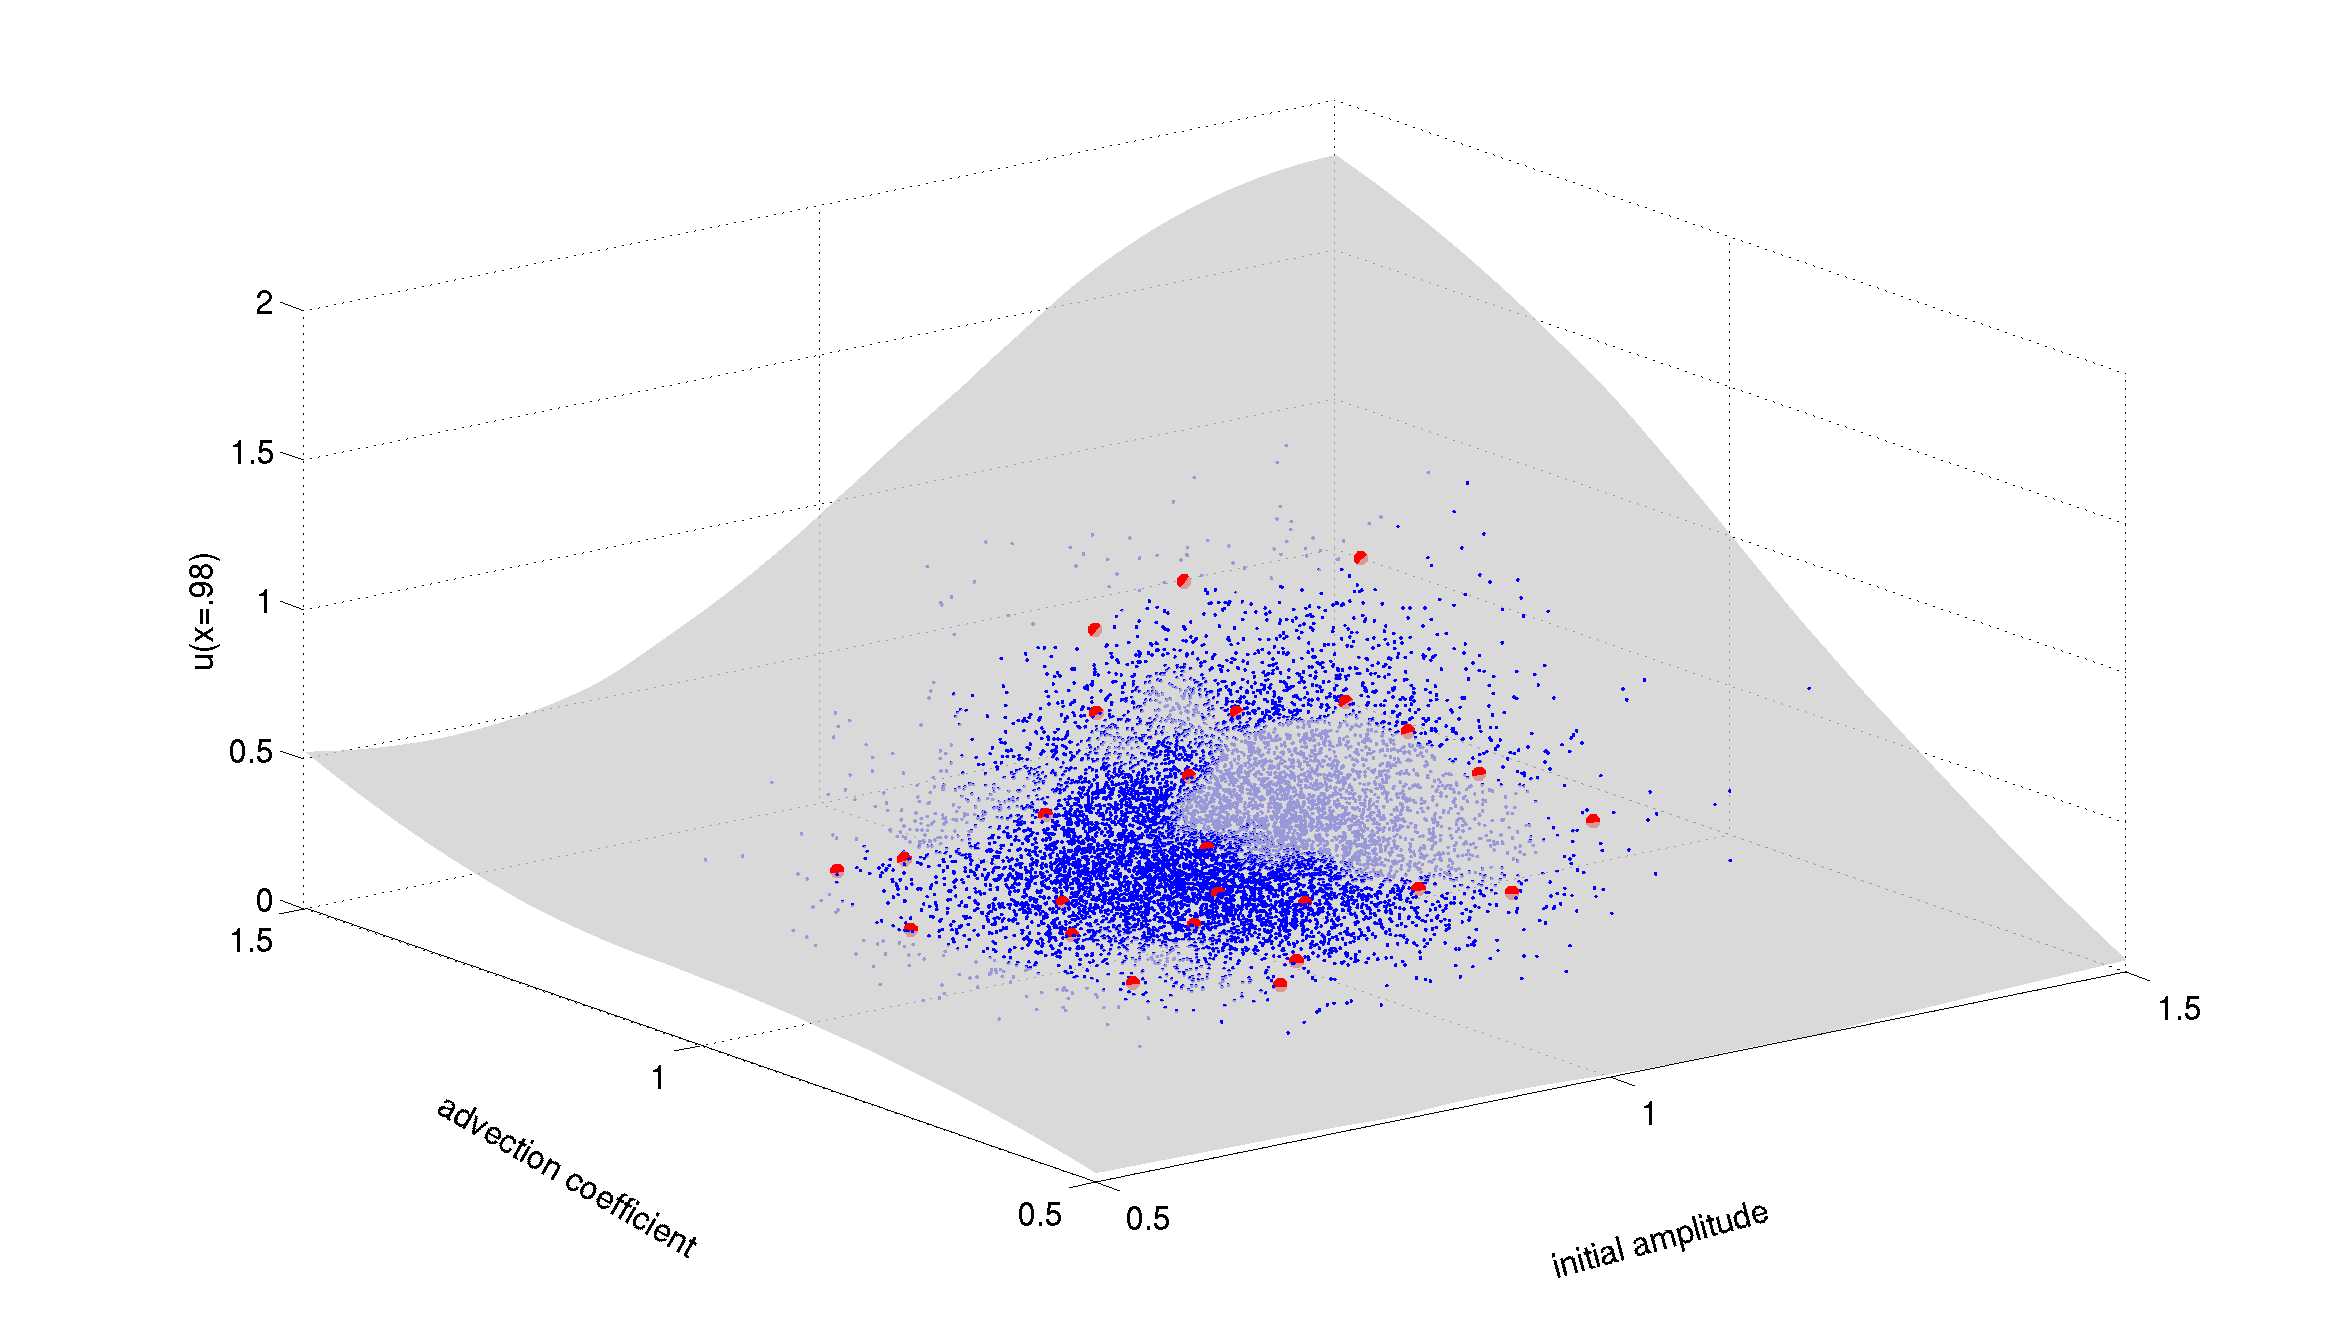
\includegraphics[width=.8\textwidth]{gasp_burger.png}
\end{figure}

\end{frame}
\end{withoutheadline}
%=============================================================
\begin{withoutheadline}
\begin{frame}\frametitle{Case 1: Results} 


\center{Emulator result + error}
\begin{figure}
\center 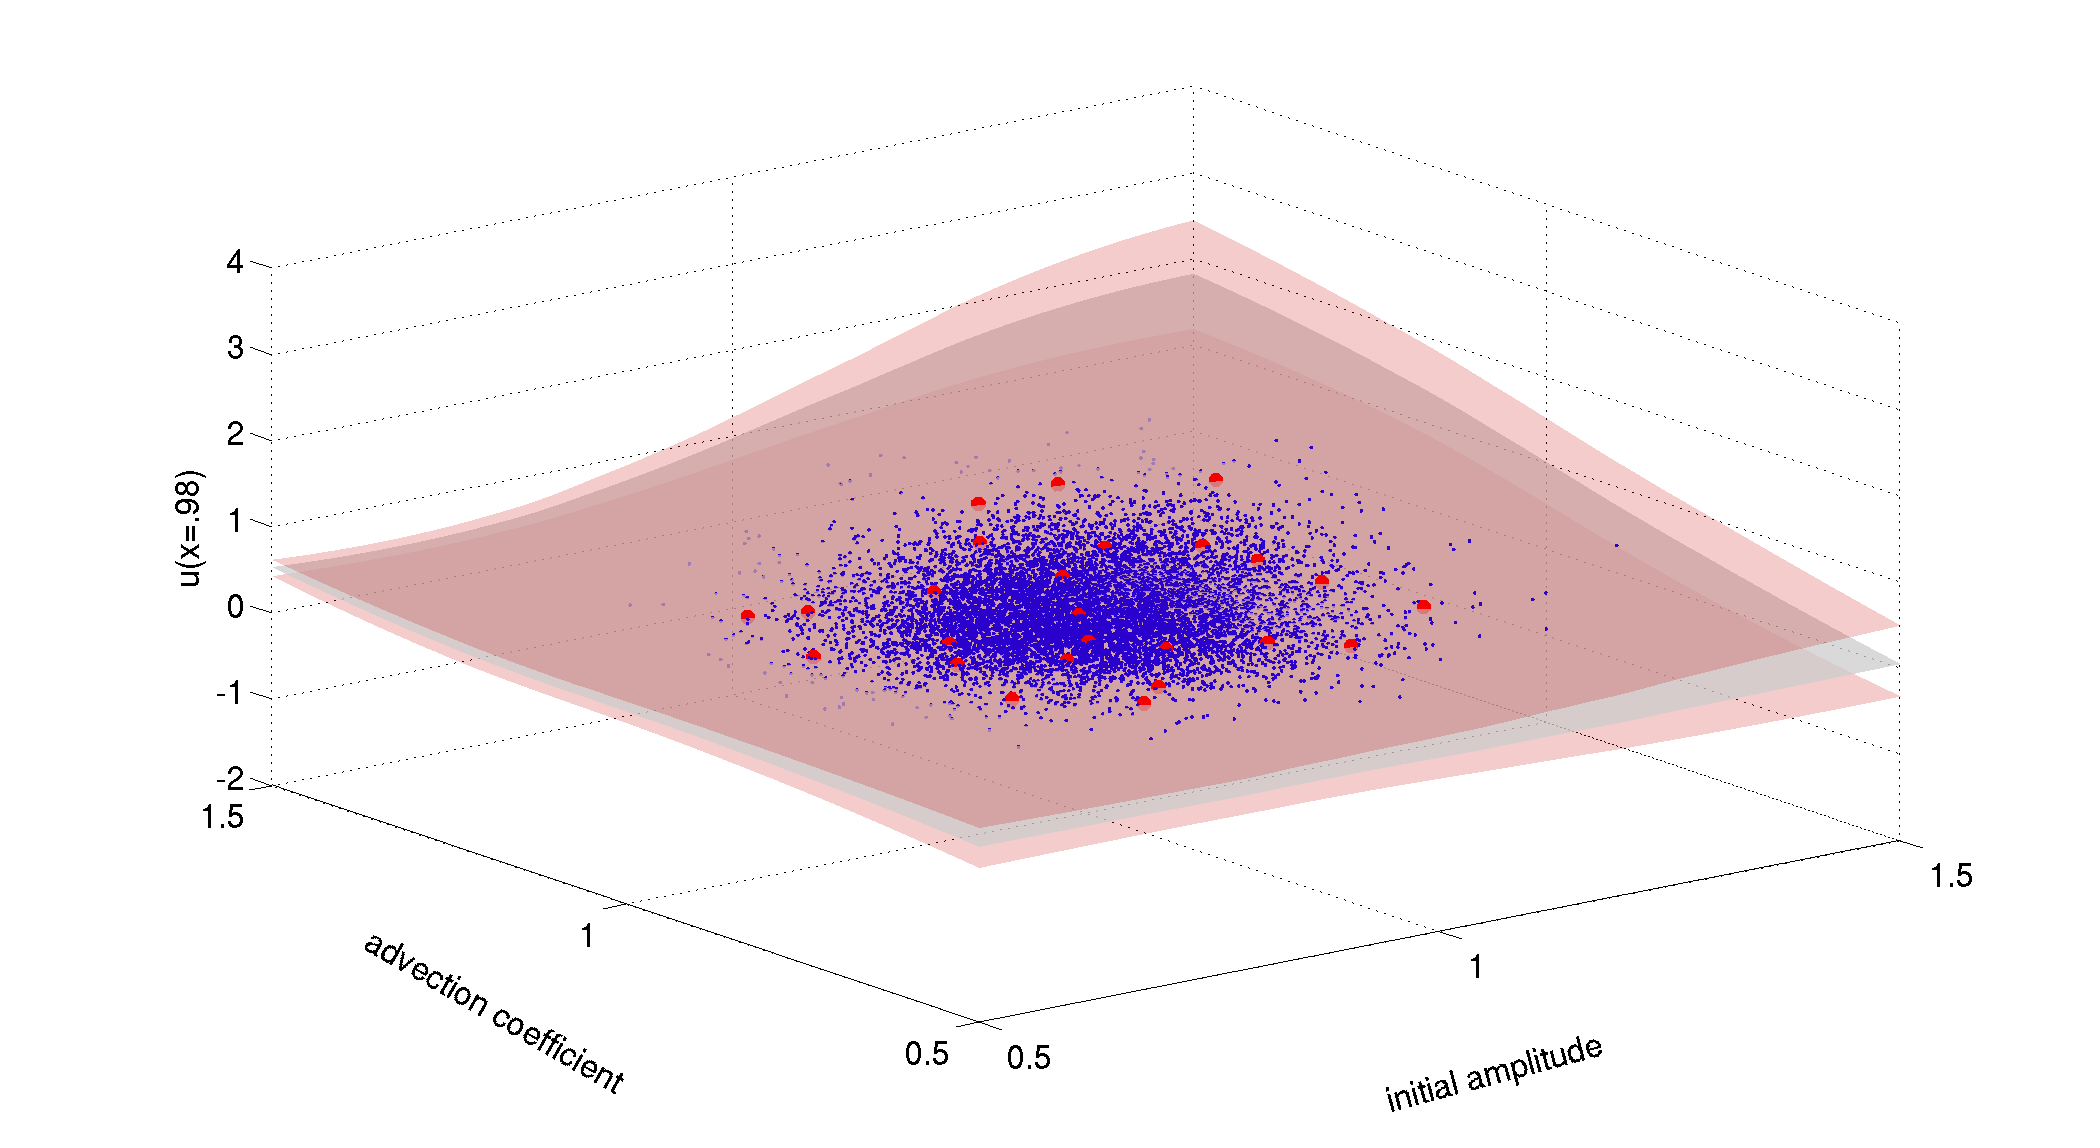
\includegraphics[width=.8\textwidth]{gasp_burger_err.png}
\end{figure}

\end{frame}
\end{withoutheadline}
%=============================================================
\begin{withoutheadline}
\begin{frame} 
\frametitle{Governing Equations}

\begin{displaymath}
 \large{U_t + F(U)_x + G(U)_y = S(U)}
\end{displaymath}

Where:
\begin{displaymath}
\begin{aligned}
U & = (h, hv_x, hv_y)^T \\
F & = (hv_x, hv_x^2+0.5k_{ap}g_zh^2, hv_xhv_y)^T \\
G & = (hv_y, hv_xv_y, hv_y^2+0.5k_{ap}g_zh^2)^T \\
\end{aligned}
\end{displaymath}
\end{frame}
\end{withoutheadline}
%=============================================================
\begin{withoutheadline}
\begin{frame} 
\frametitle{Governing Equations Cont.}
\begin{displaymath}
\begin{aligned}
S & = (0, S_x, S_y)^T \\
S_x & = g_x h  - \frac{V_x}{\sqrt{V_x^2+V_y^2}}\left(g_z h+\frac{hV_x^2}{r_x}\right)\tan(\phi_{bed}) \\
 & - h k_{ap}{\rm sgn}\left({\frac{\partial V_x}{\partial y}}\right) \frac{\partial (g_zh)}{\partial y} \sin(\phi_{int})\\
S_y & = g_y h  - \frac{V_y}{\sqrt{V_x^2+V_y^2}}\left(g_z h+\frac{hV_y^2}{r_y}\right)\tan(\phi_{bed}) \\
 & - h k_{ap}{\rm sgn}\left({\frac{\partial V_y}{\partial x}}\right) \frac{\partial (g_zh)}{\partial x} \sin(\phi_{int})
\end{aligned}
\end{displaymath}
\end{frame}
\end{withoutheadline}
%=============================================================

\begin{withoutheadline}
\begin{frame}\frametitle{Results} 


\end{frame}
\end{withoutheadline}
%=============================================================
\begin{withoutheadline}
\begin{frame}\frametitle{Sensitivity Computation} 


\end{frame}
\end{withoutheadline}
%=============================================================
\begin{withoutheadline}
\begin{frame}\frametitle{Sensitivity Computation} 


\end{frame}
\end{withoutheadline}
%=============================================================
\begin{withoutheadline}
\begin{frame}\frametitle{Sensitivity Computation} 


\end{frame}
\end{withoutheadline}
%=============================================================
\begin{withoutheadline}
\begin{frame}\frametitle{Sensitivity Computation} 


\end{frame}
\end{withoutheadline}
%=============================================================
\begin{withoutheadline}
\begin{frame}\frametitle{Sensitivity Computation} 


\end{frame}
\end{withoutheadline}
%============================================================
%Appendix
%=============================================================
\appendix
\section{More}
\begin{frame}[label=supplemental]
\frametitle{Connection to Adjoint definition} 

\begin{equation}
    \begin{aligned}
  u&= \frac{d U}{d \alpha}, \hspace{.3 in} A&=\ \frac{\partial R}{\partial U} 
 \\ g^T&= \frac{\partial J}{\partial U},  \hspace{.3 in} f&=-\frac{\partial R}{\partial \alpha}
 \end{aligned}
   \end{equation}

   Forward method:
   \begin{equation}
   \label{disadj1}
      \begin{aligned}
  \frac{dJ}{d \alpha} = g^T u + \frac{\partial J}{\partial \alpha} \\
   \text{Subject to} \hspace{.15 in} Au = f
     \end{aligned}
  \end{equation}

  Adjoint Method:
  
  \begin{equation}
   \label{disadj2}
      \begin{aligned}
  \frac{dJ}{d \alpha} = v^T f + \frac{\partial J}{\partial \alpha} \\
   \text{Subject to} \hspace{.15 in} A^T v = g
     \end{aligned}
 \end{equation}

Back to \hyperlink{main}{\beamerbutton{Connection adjoint definition}}.
\end{frame}
%\subsection{Subsection no.1.1  }
%\begin{frame} 
%Without title somethink is missing. 
%\end{frame}
%
%
%
%\section{Section no. 2} 
%\subsection{Lists I}
%\begin{frame}\frametitle{unnumbered lists}
%\begin{itemize}
%\item Introduction to  \LaTeX  
%\item Course 2 
%\item Termpapers and presentations with \LaTeX 
%\item Beamer class
%\end{itemize} 
%\end{frame}
%
%\begin{frame}\frametitle{lists with pause}
%\begin{itemize}
%\item Introduction to  \LaTeX \pause 
%\item Course 2 \pause 
%\item Termpapers and presentations with \LaTeX \pause 
%\item Beamer class
%\end{itemize} 
%\end{frame}
%
%\subsection{Lists II}
%\begin{frame}\frametitle{numbered lists}
%\begin{enumerate}
%\item Introduction to  \LaTeX  
%\item Course 2 
%\item Termpapers and presentations with \LaTeX 
%\item Beamer class
%\end{enumerate}
%\end{frame}
%
%\begin{frame}\frametitle{numbered lists with pause}
%\begin{enumerate}
%\item Introduction to  \LaTeX \pause 
%\item Course 2 \pause 
%\item Termpapers and presentations with \LaTeX \pause 
%\item Beamer class
%\end{enumerate}
%\end{frame}
%
%\section{Section no.3} 
%\subsection{Tables}
%\begin{frame}\frametitle{Tables}
%\begin{tabular}{|c|c|c|}
%\hline
%\textbf{Date} & \textbf{Instructor} & \textbf{Title} \\
%\hline
%WS 04/05 & Sascha Frank & First steps with  \LaTeX  \\
%\hline
%SS 05 & Sascha Frank & \LaTeX \ Course serial \\
%\hline
%\end{tabular}
%\end{frame}
%
%
%\begin{frame}\frametitle{Tables with pause}
%\begin{tabular}{c c c}
%A & B & C \\ 
%\pause 
%1 & 2 & 3 \\  
%\pause 
%A & B & C \\ 
%\end{tabular} 
%\end{frame}
%
%
%\section{Section no. 4}
%\subsection{blocs}
%\begin{frame}\frametitle{blocs}
%
%\begin{block}{title of the bloc}
%bloc text
%\end{block}
%
%\begin{exampleblock}{title of the bloc}
%bloc text
%\end{exampleblock}
%
%
%\begin{alertblock}{title of the bloc}
%bloc text
%\end{alertblock}
%\end{frame}
%
%\section{Section no. 5}
%\subsection{split screen}
%
%\begin{frame}\frametitle{splitting screen}
%\begin{columns}
%\begin{column}{5cm}
%\begin{itemize}
%\item Beamer 
%\item Beamer Class 
%\item Beamer Class Latex 
%\end{itemize}
%\end{column}
%\begin{column}{5cm}
%\begin{tabular}{|c|c|}
%\hline
%\textbf{Instructor} & \textbf{Title} \\
%\hline
%Sascha Frank &  \LaTeX \ Course 1 \\
%\hline
%Sascha Frank &  Course serial  \\
%\hline
%\end{tabular}
%\end{column}
%\end{columns}
%\end{frame}
%
%\subsection{Pictures} 
%\begin{frame}\frametitle{pictures in latex beamer class}
%\begin{figure}
%\includegraphics[scale=0.1]{/home/hossein/Pictures/Yandex-Images-2015-02-22.jpg} 
%\caption{show an example picture}
%\end{figure}
%\end{frame}
%
%\subsection{joining picture and lists} 
%
%\begin{frame}
%\frametitle{pictures and lists in beamer class}
%\begin{columns}
%\begin{column}{5cm}
%\begin{itemize}
%\item<1-> subject 1
%\item<3-> subject 2
%\item<5-> subject 3
%\end{itemize}
%\vspace{3cm} 
%\end{column}
%\begin{column}{5cm}
%\begin{overprint}
%\includegraphics<2>[scale=0.1]{/home/hossein/Pictures/Yandex-Images-2015-02-22.jpg}
%\includegraphics<4>[scale=0.1]{/home/hossein/Pictures/Yandex-Images-2015-02-22.jpg}
%\includegraphics<6>[scale=0.1]{/home/hossein/Pictures/Yandex-Images-2015-02-22.jpg}
%\end{overprint}
%\end{column}
%\end{columns}
%\end{frame}
%
%
%\subsection{pictures which need more space} 
%\begin{frame}[plain]
%\frametitle{plain, or a way to get more space}
%\begin{figure}
%\includegraphics[scale=0.1]{/home/hossein/Pictures/Yandex-Images-2015-02-22.jpg} 
%\caption{show an example picture}
%\end{figure}
%\end{frame}
%

\end{document}